\documentclass[a4paper,11pt]{article}

\usepackage[margin=2cm]{geometry}
\usepackage{graphicx}
\usepackage{booktabs}
\usepackage{caption}
\usepackage{mathptmx}
\usepackage{amssymb}
\usepackage{amsfonts}
\usepackage{threeparttable}
\usepackage{placeins}
\usepackage{siunitx}
\usepackage{amsmath}
\usepackage[super]{nth}

\sisetup{
    round-mode = figures,
    round-precision = 4
}

\begin{document}

\title{\Large{\textbf{Unknown Signal}}}
\author{Elan Virtucio}
\date{}
\maketitle

\section{Introduction}
It is very useful to be able to model a given set of data points to an
appropriate degree of accuracy. This can allow for predictions to be made
for an output given some input.
\\ \\
In this instance, a set of data points is given which follows an unknown
signal. The task given was to reconstruct this signal and alongside it,
calculate the sum squared error or residual sum of squares (RSS) to give an
idea of how well the model represents the data.  There are different segments
of this signal and each one can be modelled by either a linear function, a
polynomial function of a given degree or some other function that is unknown.
\\ \\
Although it's possible to model a set of data, ultimately, the results will
be highly dependent on the accuracy and correlation of the data and therefore
problems may arise such as overfitting. The aims of this project were to
minimise these effects and address the limitiations of modelling a data set.

\section{Implementation}
The program is \textit{lsr.py} and it takes in Comma Separated Value (CSV) files
consisiting two columns for the x and y data points respectively. The files can
contain one or multiple line segements and each line segments consists of 20
data points. The segments are split up and for each one, a model is fitted
and it's RSS is calculated. The RSS of each line segment are summed up to
produce the total RSS.
\\ \\
The regression method used was the matrix form of the Least Squares Regression (LSR)
and to account for any form of overfitting, the use of a k-fold cross-validation (CV)
was used. There are two implementation that can be used, a fixed k-fold
or a random k-fold. For example, if $k = 5$, in a fixed k-fold, the parts are split up
like so; $[[0, 1, 2, 3], [4, 6, 7, 8], \dots, [16, 17, 18, 19]]$ where the
numbers represent the index of the data point. Whereas, in a random k-fold, the parts
can be split up like so; $[[8, 3, 19, 7], [10, 2, 14, 4], \dots, [15, 1, 0, 8]]$,
and this can differ per run. 
\\ \\
The program iterates through a list of defined models as described in Table
\ref{tab:models} where $\hat{y}$ is the resulting regression function. These
models are a list object of their own and contains the properties that'll allow it
to model a data set using LSR. These properties are it's name, the relevant function required
to extend the $X$ vector with the relevant feature vectors, where $X$ consists of the x
data points, and additionally, the equation to use. The data is modelled using
each of this models and the RSS is calculated for each one or to be more precise,
the CV error, which corresponds to the average RSS value that was calculated
during the CV process.  The model that produced the minimum error gets chosen
as the model to use for that data set.

\begin{table}[ht!]
    \centering
    \begin{threeparttable}
    \caption{Models}
    \label{tab:models}
    \begin{tabular}{l c c}
        \toprule
        Name & $X$ & $\hat{y}$ \\
        \midrule
        Linear
            & $\begin{bmatrix}
                1      & x_0       \\
                \vdots & \vdots    \\
                1      & x_{N - 1} 
               \end{bmatrix}$
            & $a_0 + a_1x_i$
            \\ \\
        \nth{2} to \nth{10} Degree Polynomials
            & $\begin{bmatrix}
                1      & x_0       & \dots  & x_0^d       \\
                \vdots & \vdots    & \ddots & \vdots      \\
                1      & x_{N - 1} & \dots  & x_{N - 1}^d
                \end{bmatrix}$
            & $a_0 + a_1x_i + \dots + a_dx_i^d$
            \\ \\
        Exponential
            & $\begin{bmatrix}
                1      & e^{x_0}       \\
                \vdots & \vdots        \\
                1      & e^{x_{N - 1}}
               \end{bmatrix}$
            & $a_0 + a_1e^{x_i}$
            \\ \\
        Sinusoidal
            & $\begin{bmatrix}
                1      & sin(x_0)       \\
                \vdots & \vdots         \\
                1      & sin(x_{N - 1}) 
               \end{bmatrix}$
            & $a_0 + a_1sin(x_i)$
            \\ \\
        Cosinusoidal
            & $\begin{bmatrix}
                1      & cos(x_0)       \\
                \vdots & \vdots         \\
                1      & cos(x_{N - 1})
               \end{bmatrix}$
            & $a_0 + a_1cos(x_i)$
            \\ \\
        \bottomrule
    \end{tabular}
    \begin{tablenotes}
        \item[1] $N =$ \textit{number of data points} $\ \therefore \  N = 20$.
        \\
        \item[2] $a_j \in A = (X^T X)^{-1}XY \ \mid \  Y = \begin{bmatrix}y_0 \\ \vdots \\ y_{N - 1}\end{bmatrix}$ 
        \\
        \item[3] $d \in \mathbb{N} \ \mid \ 2 \ \leq \  d \  \leq \  10$
        \\
        \item[4] $i \in \mathbb{Z} \ \mid \ 0 \ \leq \  i \  < \  N$
    \end{tablenotes}
    \end{threeparttable}
\end{table}

\FloatBarrier

    \subsection{Running the Program}
    \textit{lsr.py} takes in CSV files as arguments. There are other optional
    arguments that can be passed: \texttt{--plot} shows a visual plot of the
    fitted line, \texttt{-k=10} uses 10 as the value for k in the k-fold CV process,
    \texttt{-v} makes the output more verbose by outputting the model that was
    used per line segment, \texttt{--random-k-fold} uses the random implementation
    of k-fold CV, \texttt{--no-cross-validation} runs the program without using CV.

\section{Results}
The following results that will be mentioned were obtained using the lab machines.
There were multiple different runs of the program accross all of the train data
files that were provided. This included changing the k-fold CV methods used including
changing the k values as well running it without CV. With these runs, it was
surmised that the three function types that were used were linear, cubic and sinusoidal.
This was because across all of the basic train files provided, these were the models
that the program fitted consistently and additionally, they visually produced
acceptable fits for the data. There were other models that were fitted with the
advance and noise files, however, considering the specification of the project of
having only a linear, a polynomial of a fixed degree, and some additional function
in the line segments, these were ruled out as cases of overfitting.
\\ \\
These redundant models were then commented out for future runs of the program
and therefore were not part of the iteration of the list of models to fit the data
in. An instance of this is shown in Table \ref{tab:result1}

\begin{table}[ht!]
    \scriptsize
    \centering
    \caption{Results of training data files using a fixed 10-fold CV}
    \label{tab:main_results}
    \begin{tabular}{l l l}
        \toprule
        File (.csv) & RSS & Fitted Models \textit{w.r.t.} the Line Segments \\
        \midrule
        basic\_1
            & \num{2.22853205725e-27}
            & Linear
        \\
        basic\_2
            & \num{2.0549826581e-27}
            & Linear, Linear
        \\
        basic\_3
            & \num{3.80497072739e-18}
            & Cubic
        \\
        basic\_4
            & \num{8.64481149963e-11}
            & Linear, Cubic
        \\
        basic\_5
            & \num{2.15680882375e-25}
            & Sinusoidal
        \\
        adv\_1
            & \num{220.445220441}
            & Sinusoidal, Linear, Cubic
        \\
        adv\_2
            & \num{3.68513205045}
            & Sinusoidal, Linear, Sine
        \\
        adv\_3
            & \num{1019.02994947}
            & Sinusoidal, Cubic, Sinusoidal, Linear, Sinusoidal, Cubic
        \\
        noise\_1
            & \num{12.2074601401}
            & Linear
        \\
        noise\_2
            & \num{849.552746233}
            & Linear, Cubic
        \\
        noise\_3
            & \num{482.909050785}
            & Linear, Cubic, Sinusoidal
        \\
        \bottomrule
    \end{tabular}
\end{table}

\FloatBarrier

\begin{table}[ht!]
    \begin{minipage}{0.5\linewidth}
    \scriptsize
    \centering
    \caption{Results of noise training data files without CV}
    \label{tab:noise_no_cv_results}
    \begin{tabular}{l l l}
        \toprule
        File (.csv) & RSS & Fitted Models \textit{w.r.t.} the Line Segments \\
        \midrule
        noise\_1
            & \num{10.9850554645}
            & Cubic
        \\
        noise\_2
            & \num{797.916656822}
            & Cubic, Cubic
        \\
        noise\_3
            & \num{477.699338119}
            & Cubic, Cubic, Sinusoidal
        \\
        \bottomrule
    \end{tabular}
    \end{minipage}
    \begin{minipage}{0.5\linewidth}
    \centering
    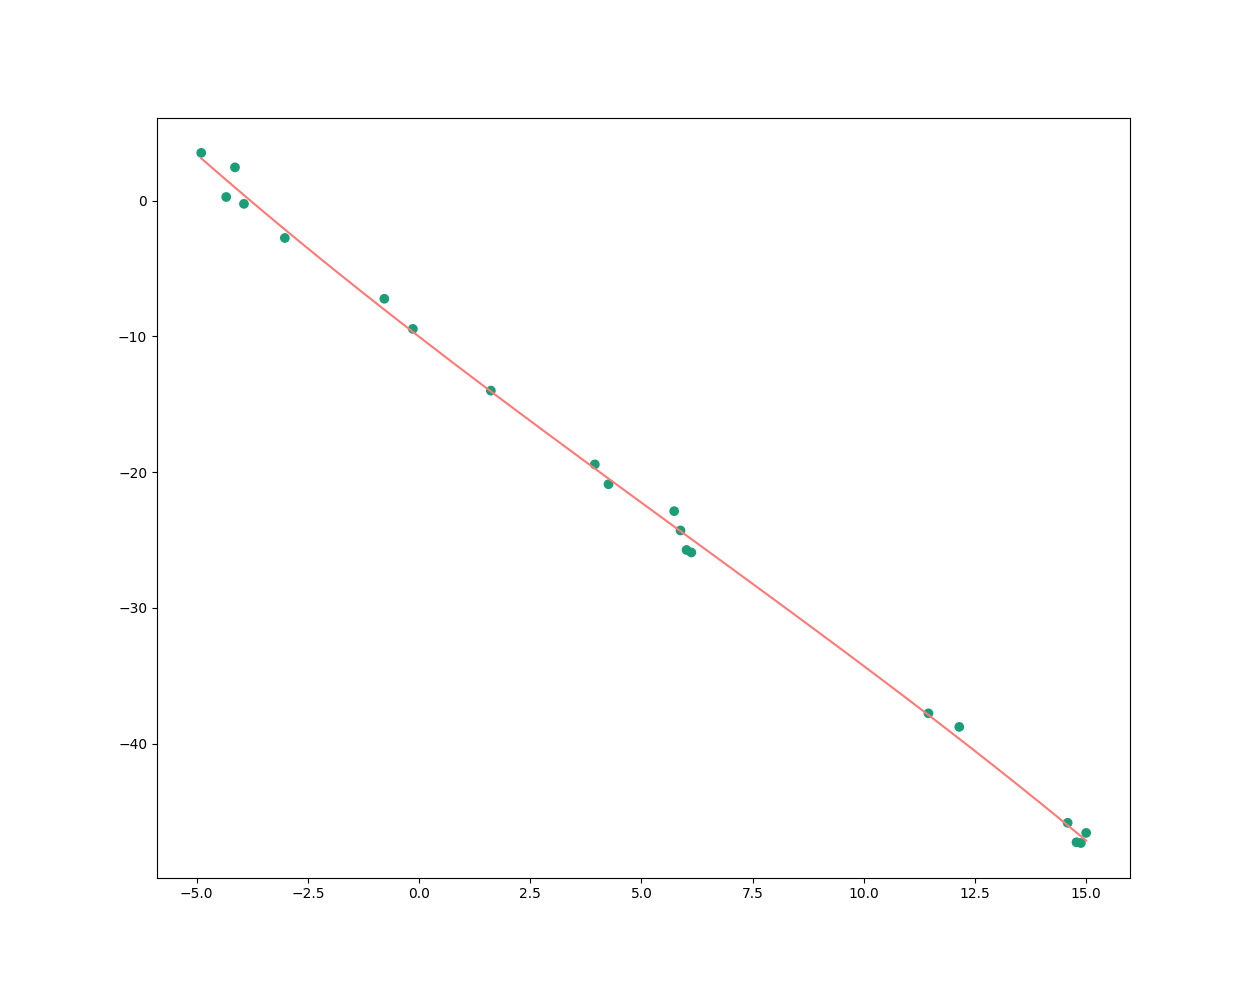
\includegraphics[width=1\linewidth]{res/noise_1_no_cv.png}
    \captionof{figure}{Plot of fitted line of \textit{noise\_1.csv} from Table \ref{tab:noise_no_cv_results}}
    \label{fig:noise_1_no_cv}
    \end{minipage}
\end{table}

\FloatBarrier

\begin{table}[ht!]
    \begin{minipage}{0.5\linewidth}
    \scriptsize
    \centering
    \caption{Results of multiple runs of adv\_3.csv using a random 5-fold CV}
    \label{tab:result1}
    \begin{tabular}{l l l}
        \toprule
        Run & RSS & Fitted Models \textit{w.r.t.} the Line Segments \\
        \midrule
        1
            & \num{1020.76902787}
            & Linear, Cubic, Sinusoidal, Linear, Sinusoidal, Cubic
        \\
        2
            & \num{1008.18577729}
            & Linear, Cubic, Sinusoidal, Cubic, Sinusoidal, Cubic
        \\
        3
            & \num{993.507417746}
            & Cubic, Cubic, Sinusoidal, Linear, Sinusoidal, Cubic
        \\
        4
            & \num{1019.02994947}
            & Sinusoidal, Cubic, Sinusoidal, Linear, Sinusoidal, Cubic
        \\
        5
            & \num{1019.02994947}
            & Sinusoidal, Cubic, Sinusoidal, Linear, Sinusoidal, Cubic
        \\
        6
            & \num{1006.4466989}
            & Sinusoidal, Cubic, Sinusoidal, Cubic, Sinusoidal, Cubic
        \\
        7
            & \num{1006.4466989}
            & Sinusoidal, Cubic, Sinusoidal, Cubic, Sinusoidal, Cubic
        \\
        8
            & \num{1020.76902787}
            & Linear, Cubic, Sinusoidal, Linear, Sinusoidal, Cubic
        \\
        9
            & \num{1008.18577729}
            & Linear, Cubic, Sinusoidal, Cubic, Sinusoidal, Cubic
        \\
        10
            & \num{1019.02994947}
            & Sinusoidal, Cubic, Sinusoidal, Linear, Sinusoidal, Cubic
        \\
        \bottomrule
    \end{tabular}
    \end{minipage}
    \begin{minipage}{0.5\linewidth}
    \centering
    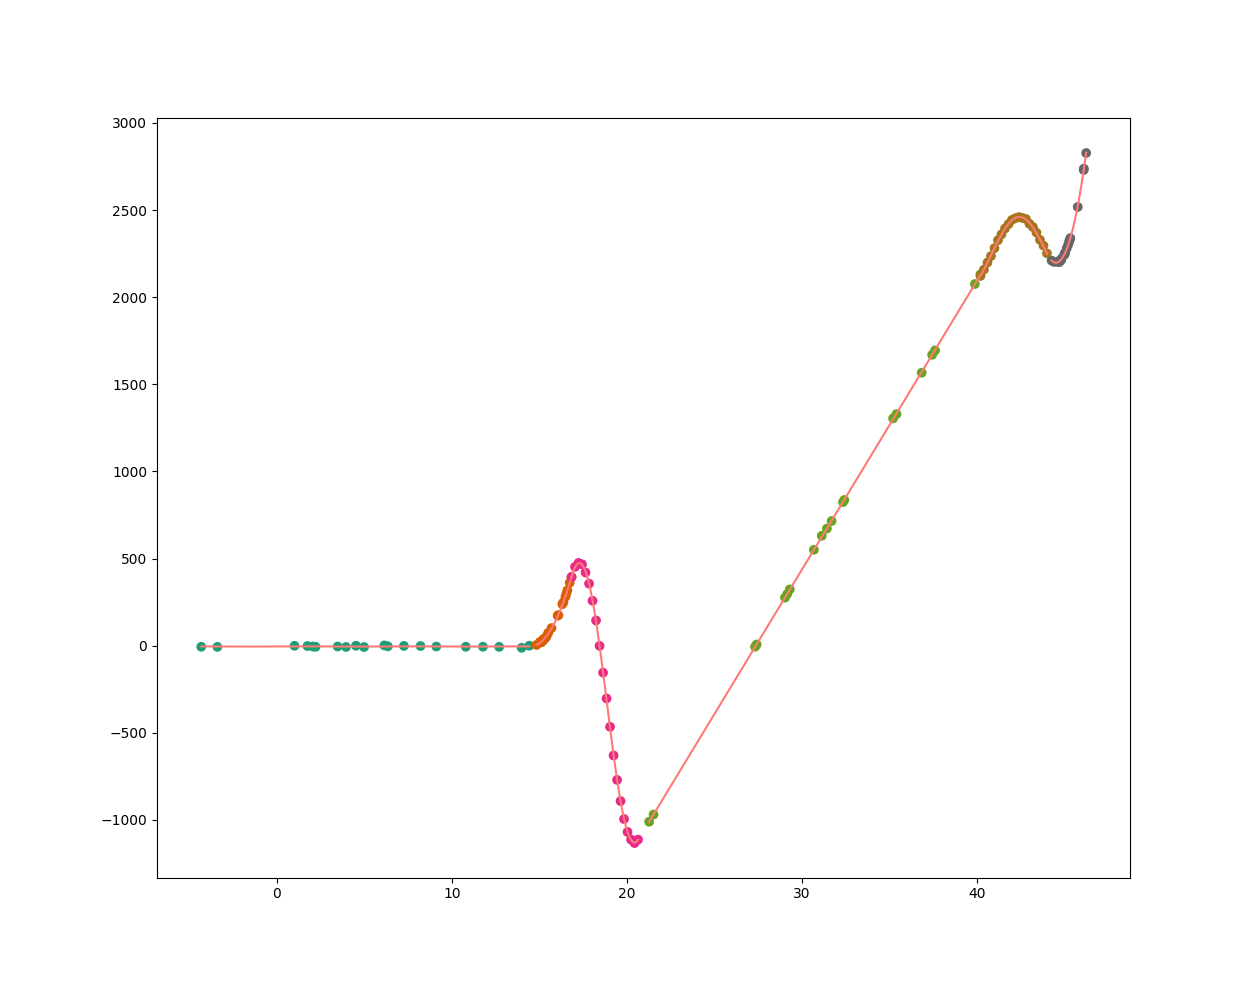
\includegraphics[width=1\linewidth]{res/adv_3.png}
    \captionof{figure}{Plot of fitted line of \textit{adv\_3.csv} from Table \ref{tab:main_results}}
    \label{fig:noise_1_no_cv}
    \end{minipage}
\end{table}

\FloatBarrier
\section{Conclusion}

\end{document}
